\documentclass[10pt]{article}

\usepackage[letterpaper,margin=0.68in]{geometry}
\usepackage[T1]{fontenc}
\usepackage{lmodern}
\usepackage{microtype}
\usepackage{amsmath,amssymb}
\usepackage{graphicx}
\usepackage{booktabs}
\usepackage{tabularx}
\usepackage{array}
\usepackage{enumitem}
\usepackage{xcolor}
\usepackage{tikz}
\usetikzlibrary{arrows.meta,positioning,fit,calc}
\usepackage{caption}
\usepackage[hidelinks]{hyperref}

\definecolor{CaptureBlue}{HTML}{377EB8}
\definecolor{GeometryTeal}{HTML}{149C95}
\definecolor{EvidenceOrange}{HTML}{E68632}
\definecolor{ModePurple}{HTML}{7B5FC6}
\definecolor{SoftGray}{HTML}{F2F4F6}
\definecolor{DarkGray}{HTML}{30343B}

\hypersetup{
  pdftitle={Recovering 3D Vibration Modes from Multi-View Videos with Gaussian Splatting},
  colorlinks=true,
  linkcolor=ModePurple,
  citecolor=ModePurple,
  urlcolor=CaptureBlue
}

\setlength{\parindent}{0pt}
\setlength{\parskip}{0.45em}
\setlist[itemize]{leftmargin=1.35em,itemsep=0.2em,topsep=0.25em}
\captionsetup{font=small,labelfont=bf}

\newcommand{\plainidea}[1]{%
  \vspace{0.25em}
  \noindent\colorbox{SoftGray}{%
    \parbox{\dimexpr\linewidth-2\fboxsep\relax}{%
      \textbf{Plain-language idea.} #1}}
  \vspace{0.25em}
}

\newcommand{\technicaldetail}[1]{%
  \vspace{0.25em}
  \noindent\fcolorbox{ModePurple}{white}{%
    \parbox{\dimexpr\linewidth-2\fboxsep-2\fboxrule\relax}{%
      \small\textbf{Technical detail.} #1}}
  \vspace{0.25em}
}

\newcommand{\figureplaceholder}[3]{%
  \begin{figure}[htbp]
    \centering
    \IfFileExists{#1}{%
      \includegraphics[width=#2\linewidth]{#1}
    }{%
      \fcolorbox{DarkGray}{SoftGray}{%
        \parbox[c][0.20\textheight][c]{\dimexpr#2\linewidth-2\fboxsep-2\fboxrule\relax}{%
          \centering\small\textbf{Figure placeholder}\\[0.5em]
          \texttt{\detokenize{#1}}\\[0.5em]
          See \texttt{figures/README.md} for the requested Bush asset.}}
    }
    \caption{#3}
  \end{figure}
}

\newcommand{\stagebox}[4]{%
  \node[draw=#1, very thick, rounded corners=2pt, fill=#1!7,
        minimum height=1.05cm, text width=2.45cm, align=center,#4] (#2) {#3};}

\begin{document}

{\Huge\bfseries Recovering 3D Vibration Modes from Multi-View Videos\\
with Gaussian Splatting\par}
\vspace{0.35em}
{\large An accessible technical brief for an internal research poster\par}
\vspace{0.7em}
\hrule
\vspace{0.7em}

\textbf{One-sentence objective.}
Given one video that scans a stationary object and several fixed-camera videos
that record its vibration, recover a set of spatially coherent \emph{3D motion
patterns} attached to a Gaussian-splat representation of the object.

\plainidea{A camera only observes motion in an image plane. We combine several
views, a shared 3D scene, and simple local shape constraints to infer how the
object could have moved in three dimensions.}

This brief follows the Bush experiment from capture through the completed
spatial 3D mode fields.

\section{Pipeline at a glance}

The method separates \emph{what the scene looks like} from \emph{how it
vibrates}. The sweep video builds a canonical static scene. The fixed cameras
then provide image-space motion evidence. A shared camera coordinate system
connects those two halves.

\begin{figure}[htbp]
  \centering
  \resizebox{\linewidth}{!}{%
  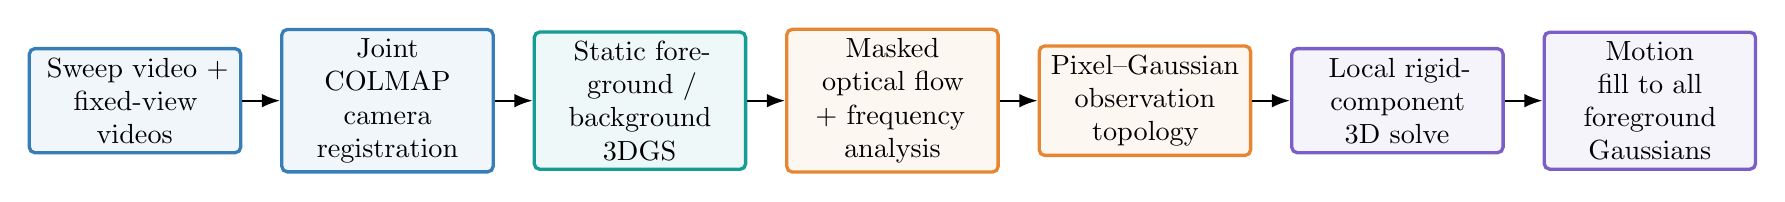
\begin{tikzpicture}[node distance=0.55cm and 0.48cm, >=Latex]
    \stagebox{CaptureBlue}{capture}{Sweep video +\\fixed-view videos}{at={(0,0)}}
    \stagebox{CaptureBlue}{colmap}{Joint COLMAP\\camera registration}{right=of capture}
    \stagebox{GeometryTeal}{static}{Static foreground /\\background 3DGS}{right=of colmap}
    \stagebox{EvidenceOrange}{flow}{Masked optical flow\\+ frequency analysis}{right=of static}
    \stagebox{EvidenceOrange}{observe}{Pixel--Gaussian\\observation topology}{right=of flow}
    \stagebox{ModePurple}{rigid}{Local rigid-component\\3D solve}{right=of observe}
    \stagebox{ModePurple}{fill}{Motion fill to all\\foreground Gaussians}{right=of rigid}
    \draw[->,thick] (capture) -- (colmap);
    \draw[->,thick] (colmap) -- (static);
    \draw[->,thick] (static) -- (flow);
    \draw[->,thick] (flow) -- (observe);
    \draw[->,thick] (observe) -- (rigid);
    \draw[->,thick] (rigid) -- (fill);
  \end{tikzpicture}}
  \caption{The Bush pipeline. Blue stages establish cameras, teal stages build
  the static 3D scene, orange stages extract image evidence, and purple stages
  recover a complete 3D mode.}
\end{figure}

The central design choice is to keep two graph-like structures separate:

\begin{itemize}
  \item an \textbf{observation topology}, which says which visible Gaussians
  contributed to measured image pixels; and
  \item a \textbf{structure graph}, which says which nearby Gaussians probably
  belong to the same local piece of the physical plant.
\end{itemize}

The first connects measurements to unknown motion. The second makes the
otherwise ambiguous 3D inference spatially coherent.

\section{What is a 3D Gaussian Splat?}

A 3D Gaussian Splatting (3DGS) scene is a collection of many small,
semi-transparent, oriented 3D ellipsoids \cite{kerbl2023gaussians}. Each
Gaussian stores a center, shape, opacity, and color. To render an image, the
camera projects the ellipsoids into 2D ``splats'' and blends them from front to
back.

More precisely, Gaussian $g$ is parameterized as
\begin{equation}
  \mathcal G_g=(\mu_g,q_g,s_g,o_g,c_g),
  \qquad
  \mu_g\in\mathbb R^3,
  \quad s_g\in\mathbb R_{>0}^3,
  \quad o_g\in(0,1),
  \quad c_g\in[0,1]^3.
\end{equation}
Here $\mu_g$ is the world-space center, $q_g$ is a unit quaternion, $s_g$ is
the three-axis scale, $o_g$ is opacity, and $c_g$ is RGB color. The Bush
experiment uses direct view-independent color rather than spherical harmonics.
The implementation maintains unconstrained trainable values and applies
\begin{equation}
  q_g=\frac{\widetilde q_g}{\lVert\widetilde q_g\rVert_2},
  \qquad s_g=\exp(\widetilde s_g),
  \qquad o_g=\operatorname{sigmoid}(\widetilde o_g),
  \qquad c_g=\operatorname{sigmoid}(\widetilde c_g),
\end{equation}
which enforces the domains shown above during optimization.
The quaternion and scale define a symmetric positive-definite covariance
\begin{equation}
  \Sigma_g
  =R(q_g)\operatorname{diag}(s_g^2)R(q_g)^\top,
\end{equation}
so the unnormalized spatial density of the primitive is
\begin{equation}
  G_g(x)
  =\exp\!\left[
    -\frac{1}{2}(x-\mu_g)^\top\Sigma_g^{-1}(x-\mu_g)
  \right].
\end{equation}

\plainidea{Think of the scene as a cloud of tiny, colored, translucent stickers
floating in 3D. Seen together from a camera, they form a sharp image. Unlike a
plain video, every sticker has an explicit 3D location, so we can attach a 3D
displacement vector to it.}

\begin{figure}[htbp]
  \centering
  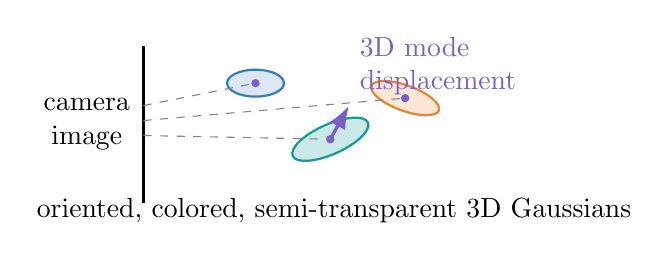
\begin{tikzpicture}[scale=0.95, >=Latex]
    \draw[very thick] (-0.3,-1.05) -- (-0.3,1.05);
    \node[align=center,left] at (-0.35,0) {camera\\image};
    \draw[fill=CaptureBlue!18,draw=CaptureBlue,thick] (1.2,0.55) ellipse (0.38 and 0.18);
    \draw[fill=GeometryTeal!22,draw=GeometryTeal,thick,rotate around={24:(2.2,-0.2)}]
      (2.2,-0.2) ellipse (0.55 and 0.20);
    \draw[fill=EvidenceOrange!20,draw=EvidenceOrange,thick,rotate around={-20:(3.2,0.35)}]
      (3.2,0.35) ellipse (0.48 and 0.17);
    \fill[ModePurple] (1.2,0.55) circle (1.6pt);
    \fill[ModePurple] (2.2,-0.2) circle (1.6pt);
    \fill[ModePurple] (3.2,0.35) circle (1.6pt);
    \draw[->,ModePurple,very thick] (2.2,-0.2) -- ++(0.25,0.45)
      node[above right,align=left] {3D mode\\displacement};
    \draw[dashed,DarkGray!60] (-0.3,0.25) -- (1.2,0.55);
    \draw[dashed,DarkGray!60] (-0.3,-0.15) -- (2.2,-0.2);
    \draw[dashed,DarkGray!60] (-0.3,0.05) -- (3.2,0.35);
    \node[align=center] at (2.25,-1.15) {oriented, colored, semi-transparent 3D Gaussians};
  \end{tikzpicture}
  \caption{A conceptual 3DGS scene. The Gaussian centers provide explicit 3D
  locations on which the recovered motion field can live.}
\end{figure}

\paragraph{Projection into one camera.}
Let a calibrated view $v$ have world-to-camera rotation $R_v$, translation
$t_v$, and pinhole intrinsics $(f_x,f_y,c_x,c_y)$. For
$x^{\mathrm c}=(x,y,z)^\top=R_vx+t_v$, its pixel projection is
\begin{equation}
  \pi_v(x^{\mathrm c})
  =
  \begin{bmatrix}
    f_x x/z+c_x\\
    f_y y/z+c_y
  \end{bmatrix}.
\end{equation}
The projected Gaussian mean and the world-displacement-to-pixel Jacobian are
\begin{align}
  m_{v,g} &= \pi_v(R_v\mu_g+t_v),\\
  J_{v,g}
  &=
  \left.
  \frac{\partial\pi_v(R_vx+t_v)}{\partial x}
  \right|_{x=\mu_g}
  =
  \begin{bmatrix}
    f_x/z_g & 0 & -f_x x_g/z_g^2\\
    0 & f_y/z_g & -f_y y_g/z_g^2
  \end{bmatrix}R_v,
\end{align}
where $(x_g,y_g,z_g)^\top=R_v\mu_g+t_v$. Linearizing the projection maps the
3D covariance into the image plane:
\begin{equation}
  \Sigma^{2D}_{v,g}
  =J_{v,g}\Sigma_gJ_{v,g}^\top+\epsilon I_2.
\end{equation}
The small $\epsilon I_2$ term represents the rasterizer's pixel-space
low-pass regularization and keeps the footprint numerically well conditioned.

\plainidea{The center tells us where the splat appears. The projected
covariance tells us the size and orientation of its elliptical footprint. The
same Jacobian $J_{v,g}$ later converts a recovered 3D vibration vector into a
2D arrow, so the rendering and motion equations share the same camera model.}

\paragraph{Front-to-back alpha compositing.}
For pixel position $p\in\mathbb R^2$, the projected opacity contributed by
Gaussian $g$ is
\begin{equation}
  a_{v,p,g}
  =o_g\exp\!\left[
    -\frac{1}{2}(p-m_{v,g})^\top
    (\Sigma^{2D}_{v,g})^{-1}(p-m_{v,g})
  \right].
\end{equation}
Suppose the overlapping Gaussians are ordered from near to far as
$g_1,\ldots,g_M$. Their transmittance and rendered contribution weight are
\begin{equation}
  T_{v,p,i}=\prod_{j<i}(1-a_{v,p,g_j}),
  \qquad
  w^{\mathrm{render}}_{v,p,i}=T_{v,p,i}a_{v,p,g_i}.
\end{equation}
The final RGB color and accumulated foreground alpha are therefore
\begin{align}
  C_v(p)
  &=\sum_{i=1}^{M}w^{\mathrm{render}}_{v,p,i}c_{g_i}
    +\left[\prod_{j=1}^{M}(1-a_{v,p,g_j})\right]c_{\mathrm{bg}},\\
  A_v(p)
  &=\sum_{i=1}^{M}w^{\mathrm{render}}_{v,p,i}
   =1-\prod_{j=1}^{M}(1-a_{v,p,g_j}).
\end{align}
An expected foreground depth can be written as
\begin{equation}
  D_v(p)
  =\frac{\sum_iw^{\mathrm{render}}_{v,p,i}z_{v,g_i}}
  {\max(A_v(p),\epsilon)},
\end{equation}
which later provides a canonical surface point for pixel--Gaussian matching.

\plainidea{A Gaussian only contributes the light that reaches it. Nearer
Gaussians consume some transparency, so farther Gaussians are multiplied by
the remaining transmittance. This is why visibility is more informative than
simply choosing the closest 3D center.}

\paragraph{Static optimization.}
All Gaussian parameters are differentiable through projection, rasterization,
and compositing. For the current static Bush run, the active image objective is
the implementation's RGB loss
\begin{equation}
  \mathcal L_{\mathrm{RGB}}
  =0.8\,\lVert C_v-I_v\rVert_1
   +0.2\left[1-\operatorname{SSIM}(C_v,I_v)\right],
\end{equation}
evaluated over registered sweep images $I_v$. Gradient-based optimization and
adaptive Gaussian densification update the primitives so that their rendered
views reproduce the capture. Auxiliary mask and depth-loss weights are zero in
this static configuration; masks still define the foreground/background data
organization used by the pipeline.

\begin{table}[htbp]
  \centering
  \caption{Core 3DGS notation reused by the modal pipeline.}
  \begin{tabularx}{\linewidth}{@{}>{$}l<{$}X@{}}
    \toprule
    \text{Symbol} & \text{Meaning} \\
    \midrule
    \mu_g,\Sigma_g & World-space mean and covariance of Gaussian $g$. \\
    q_g,s_g & Quaternion orientation and positive principal-axis scales. \\
    o_g,c_g & Gaussian opacity and RGB color. \\
    K_v,R_v,t_v & Camera intrinsics and world-to-camera extrinsics for view $v$. \\
    m_{v,g},\Sigma^{2D}_{v,g} & Projected 2D mean and elliptical covariance. \\
    J_{v,g} & Jacobian mapping a small world-space displacement to pixel motion. \\
    a_{v,p,g} & Gaussian $g$'s opacity footprint at pixel $p$. \\
    T_{v,p,i} & Transmittance remaining before the $i$th depth-ordered Gaussian. \\
    w^{\mathrm{render}}_{v,p,i} & Actual rasterization contribution $T_{v,p,i}a_{v,p,g_i}$. \\
    C_v(p),A_v(p),D_v(p) & Rendered RGB, accumulated alpha, and expected depth. \\
    \bottomrule
  \end{tabularx}
\end{table}

We train separate foreground and background Gaussian sets. The vibration
pipeline only assigns modes to foreground Gaussians. This separation matters:
the stationary scene can still render normally, while the plant has an
independent motion representation.

\section{Capture and a shared camera coordinate system}

The Bush capture contains two complementary types of video. This separation
between a canonical scene and video-derived motion follows the broader
representation strategy of Shape of Motion \cite{wang2025shape}, while the
present pipeline replaces its original camera/depth preprocessing with a joint
COLMAP route and introduces the multi-view modal solve described here.

\begin{itemize}
  \item A \textbf{sweep video} moves around the stationary plant. Its many
  viewpoints provide the parallax needed to reconstruct the canonical 3DGS.
  \item Several \textbf{fixed-view videos} observe the vibrating plant from
  static cameras. They contain clean temporal motion but little or no camera
  motion.
\end{itemize}

One reference frame from each fixed-view video is added to the sampled sweep
frames. COLMAP jointly estimates camera intrinsics and poses for this combined
image set \cite{schonberger2016sfm}. Consequently, the sweep cameras and all
fixed cameras are expressed in the same coordinate system.

\plainidea{If each camera made its own private 3D map, their motion clues could
not be combined. Joint registration gives every camera the same map and the
same definition of left, up, and depth.}

The registered sweep frames, their foreground masks, and the COLMAP cameras
are packaged as the static-training dataset. The fixed reference cameras are
also exported for the later observation and projection steps.

\figureplaceholder{figures/bush_capture_and_cameras.png}{0.88}{Requested Bush
asset: representative sweep and fixed-camera frames beside the registered
camera frustums around the static Gaussian scene.}

\section{Building the canonical static scene}

The static training stage optimizes Gaussian positions, shapes, opacities, and
colors so that rendered sweep views match the input images. This is a standard
photometric reconstruction problem: render the current Gaussians into a known
camera, compare with the real frame, and update the scene.

Foreground masks divide the scene into two Gaussian groups:

\begin{itemize}
  \item \textbf{Foreground}: the bush whose vibration modes will be recovered.
  \item \textbf{Background}: ground and surroundings that explain the images
  but should remain stationary.
\end{itemize}

The trained canonical checkpoint is the shared 3D reference for all later
frequencies. It is not retrained once per mode.

\figureplaceholder{figures/bush_static_3dgs.png}{0.78}{Requested Bush asset:
the trained canonical static 3DGS rendered from a novel view, optionally paired
with a sweep input frame.}

\section{Extracting 2D vibration evidence}

For each fixed camera, foreground masks restrict analysis to the bush. Dense
optical flow estimates a 2D displacement vector at every retained pixel
between frames; the current implementation uses Farneb\"ack's polynomial
expansion method \cite{farneback2003flow}. Optical flow does not know the
object's depth; it only says how image content moved horizontally and
vertically.

For a pixel trajectory $d_p(t)=(u_p(t),v_p(t))$, a temporal Fourier transform
asks how strongly that motion repeats at each frequency $f$:
\begin{equation}
  \widehat d_p(f)=\sum_t d_p(t)\,e^{-i2\pi f t}.
\end{equation}

The complex value stores both the oscillation strength and its phase in the
cycle. Frequency selection greedily chooses a compact set that explains the
spatially distributed flow spectra, rather than simply taking the largest
global peaks.

\plainidea{A complicated shaking video is treated as a mixture of simpler
rhythms. One selected frequency may emphasize one set of branches, while a
different frequency emphasizes another.}

\technicaldetail{The selected 2D Fourier field is evidence, not yet a 3D mode.
It remains camera-dependent and has no direct depth component. The following
stages solve for a single 3D field whose projections agree with the evidence
across cameras.}

\figureplaceholder{figures/bush_flow_and_frequency.png}{0.9}{Requested Bush
asset: a masked optical-flow frame, a representative power spectrum with a
selected frequency, and the corresponding complex 2D modal image.}

\section{Connecting pixels to visible Gaussians}

A measured pixel does not correspond to one obvious 3D point. Several
foreground Gaussians can overlap along its camera ray, with different opacity
and visibility. The observation topology records a compact set of plausible
Gaussian correspondences for each sampled foreground pixel in each fixed view.

The current topology deliberately uses a surface-guided approximation rather
than storing every rasterizer fragment. A canonical foreground render provides
$D_v(p)$ and $A_v(p)$. Pixels with inadequate mask support, invalid depth, or
low accumulated alpha are removed. Every retained pixel is unprojected to a
world-space surface point
\begin{equation}
  X_{v,p}
  =R_v^\top\left[
    D_v(p)K_v^{-1}\widetilde p-t_v
  \right],
  \qquad \widetilde p=(p_x,p_y,1)^\top.
\end{equation}
Nearby foreground Gaussians are preselected with a 3D KNN query and scored by
their opacity-weighted spatial Gaussian density:
\begin{equation}
  s_{v,p,g}
  =o_g\exp\!\left[
    -\frac12(X_{v,p}-\mu_g)^\top
    \Sigma_g^{-1}(X_{v,p}-\mu_g)
  \right].
\end{equation}
After keeping the strongest valid candidates, the topology stores
\begin{equation}
  \bar w_{v,p,g}
  =\frac{s_{v,p,g}}{\sum_{h\in C(v,p)}s_{v,p,h}},
  \qquad
  \sum_{g\in C(v,p)}\bar w_{v,p,g}=1,
\end{equation}
together with Gaussian index $g$, view $v$, pixel $p$, and the already defined
projection Jacobian $J_{v,g}$. These normalized scores are observation
confidence weights; they should not be confused with the exact depth-ordered
rasterization weights $w^{\mathrm{render}}$ from the 3DGS equations above.

For a small complex 3D displacement
$\phi_{k,g}\in\mathbb C^3$ at selected frequency $k$, the corresponding image
motion remains
\begin{equation}
  \widehat d^{\mathrm{pred}}_{v,k,g}
  =\alpha_{v,k}J_{v,g}\phi_{k,g},
\end{equation}
where $\alpha_{v,k}\in\mathbb C$ aligns the complex gain and phase of view $v$.

\plainidea{The foreground render anchors a pixel to a plausible 3D surface
point. Nearby Gaussians are then ranked by how strongly their 3D ellipsoids
support that point. The camera Jacobian tells us how a tiny 3D move of each
retained candidate would appear in the image.}

This topology is built once and reused across selected frequencies. The
frequency-specific data only changes the measured complex 2D displacement
$\widehat d_{v,k,p}$ at each sampled pixel.

\section{Building local rigid components}

The multi-view projection equations are still underconstrained: one camera
cannot directly reveal motion along its viewing direction, and observations
can be sparse. We therefore build a structure graph on the observed foreground
Gaussians.

\begin{figure}[htbp]
  \centering
  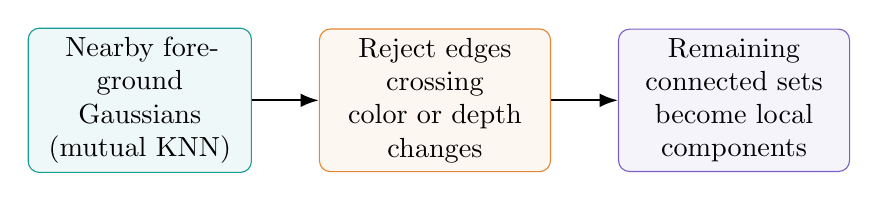
\begin{tikzpicture}[node distance=0.75cm and 0.85cm, >=Latex]
    \node[draw=GeometryTeal,fill=GeometryTeal!7,rounded corners,align=center,
      text width=2.6cm,minimum height=1.0cm] (knn) {Nearby foreground\\Gaussians (mutual KNN)};
    \node[draw=EvidenceOrange,fill=EvidenceOrange!7,rounded corners,align=center,
      text width=2.7cm,minimum height=1.0cm,right=of knn] (filter) {Reject edges crossing\\color or depth changes};
    \node[draw=ModePurple,fill=ModePurple!7,rounded corners,align=center,
      text width=2.7cm,minimum height=1.0cm,right=of filter] (components) {Remaining connected sets\\become local components};
    \draw[->,thick] (knn) -- (filter);
    \draw[->,thick] (filter) -- (components);
  \end{tikzpicture}
  \caption{Structure-graph construction. Geometry proposes local edges; color
  and rendered-depth discontinuities remove likely cross-surface links.}
\end{figure}

We begin with mutual $k$-nearest-neighbor edges in 3D. Edges are screened using
Gaussian color similarity and supporting-view rendered depth. A strong color
change or depth discontinuity suggests that two nearby Gaussians belong to
different surfaces, so that edge is removed. The connected Gaussians that
remain automatically form a local rigid component.

\plainidea{A component is not the whole bush. It is a small patch that is
allowed to translate and rotate together. Many such patches can describe
different local motions across branches and leaves.}

Tiny unsupported components are pruned, and isolated nodes remain available
for later completion rather than being silently treated as reliable rigid
parts.

\figureplaceholder{figures/bush_rigid_components.png}{0.86}{Requested Bush
asset: the observed Gaussian structure graph colored by connected component,
with the static foreground optionally shown beneath it.}

\section{Solving one 3D mode}

At each selected frequency, every reliable component receives one small
complex rigid-body motion: a translation $t_c\in\mathbb C^3$ and an angular
term $\omega_c\in\mathbb C^3$. For Gaussian $g$ in component $c$,
\begin{equation}
  \phi_{k,g}=t_c+\omega_c\times(x_g-\bar x_c),
\end{equation}
where $x_g$ is its canonical center and $\bar x_c$ is the component center.
This is a first-order motion model: it captures a small local translation and
rotation without forcing the entire plant to be one rigid object.

Define the component twist
$\xi_{k,c}=(t_{k,c}^\top,\omega_{k,c}^\top)^\top\in\mathbb C^6$ and
\begin{equation}
  B_{c,g}
  =\begin{bmatrix}I_3&-[x_g-\bar x_c]_\times\end{bmatrix},
  \qquad
  \phi_{k,g}=B_{c,g}\xi_{k,c}.
\end{equation}
The unknown twist is solved by projecting it into every supporting camera and
matching the observed complex 2D Fourier displacement. For component $c$, the
implemented weighted complex least-squares problem is
\begin{equation}
  \xi_{k,c}^{\star}
  =\underset{\xi\in\mathbb C^6}{\arg\min}
  \sum_{(v,p,g)\in\mathcal O_c}
  \bar w_{v,p,g}
  \left\|
    \alpha_{v,k}J_{v,g}B_{c,g}\xi
    -\widehat d_{v,k,p}
  \right\|_2^2.
\end{equation}
Thus each retained candidate supplies a confidence-weighted constraint that
its projected local rigid motion should match the pixel measurement. The
minimum-norm solution is computed by SVD, which also exposes rank and condition
diagnostics for deciding whether the component is a trustworthy motion seed.

\plainidea{We propose a small 3D movement for a patch, project it into each
camera, and adjust it until those projected arrows agree with the arrows
measured in the videos. Multiple views reduce the depth ambiguity.}

\technicaldetail{Complex values are bookkeeping for oscillation phase. A
global phase rotation of a mode can be exchanged with the opposite rotation of
its complex coordinate, so the absolute complex angle of $\phi_k$ alone is not
a physical orientation in 3D. The meaningful quantity is the resulting real
motion after phase and amplitude are combined.}

Components are accepted as trusted motion seeds only when their observations
provide adequate view support and numerical rank. This prevents a poorly
constrained patch from dominating later completion.

\section{Motion fill: completing the foreground}

Only some foreground Gaussians are directly observed well enough to support a
mode solve. Leaves can be occluded, masks can omit thin regions, and sampling
does not cover every Gaussian. A separate foreground KNN graph propagates
motion from trusted seeds to the remaining Gaussians.

The fill solves a smooth graph-constrained interpolation while holding trusted
seed motion fixed. A maximum graph-hop distance prevents motion from spreading
arbitrarily far across disconnected regions.

\plainidea{First solve motion where the cameras provide convincing evidence.
Then use neighboring Gaussians on the same 3D structure to fill the gaps, like
extending a partially colored drawing without repainting the known pixels.}

The output for each frequency is a complete complex field
\begin{equation}
  \phi_k\in\mathbb C^{G\times 3},
\end{equation}
with one 3D displacement vector for every foreground Gaussian. Together, the
selected fields form a reusable bank of spatial 3D vibration modes.

\figureplaceholder{figures/bush_motion_fill.png}{0.9}{Requested Bush asset:
the same mode before and after motion fill, using a consistent displacement or
phase color scale to reveal newly covered foreground Gaussians.}

\section{Qualitative Bush result}

The Bush experiment demonstrates the full intended result of this brief:
fixed-view 2D vibrations become coherent 3D displacement patterns over the
foreground Gaussian scene. Different selected frequencies emphasize different
spatial regions and phase relationships, while the static appearance remains
available for ordinary rendering.

\begin{figure}[htbp]
  \centering
  \begin{tabular}{@{}cc@{}}
    \fbox{\parbox[c][0.15\textheight][c]{0.44\linewidth}{\centering
      \textbf{Mode A}\\Bush Gaussian phase/displacement view}} &
    \fbox{\parbox[c][0.15\textheight][c]{0.44\linewidth}{\centering
      \textbf{Mode B}\\Bush Gaussian phase/displacement view}} \\[0.5em]
    \fbox{\parbox[c][0.15\textheight][c]{0.44\linewidth}{\centering
      \textbf{Mode C}\\Bush Gaussian phase/displacement view}} &
    \fbox{\parbox[c][0.15\textheight][c]{0.44\linewidth}{\centering
      \textbf{Mode D}\\Bush Gaussian phase/displacement view}}
  \end{tabular}
  \caption{Requested Bush asset: four representative recovered 3D modes,
  captured from the same camera and with consistent visualization settings.
  Replace the four boxes with labeled screenshots.}
\end{figure}

What should be inspected qualitatively:

\begin{itemize}
  \item \textbf{Spatial coherence}: neighboring Gaussians on a branch should
  move smoothly rather than flickering independently.
  \item \textbf{Local differentiation}: separate branches or leaves may have
  different amplitude and phase rather than behaving as one global rigid body.
  \item \textbf{Cross-view consistency}: a mode should remain plausible when
  viewed from different camera angles.
  \item \textbf{Coverage}: motion fill should bring most intended foreground
  Gaussians into the mode without visibly leaking into the background.
\end{itemize}

\section{What the result means---and what it does not}

The recovered $\phi_k$ fields are compact, spatially interpretable 3D motion
atoms supported by multi-view video evidence. They are useful for inspecting
where different vibration frequencies occur and for later animation or
physical modeling.

Important limitations remain:

\begin{itemize}
  \item The local rigid transform is a \textbf{first-order small-motion
  approximation}. Large finite playback is not guaranteed to preserve exact
  distances.
  \item Accuracy depends on masks, optical flow, static-camera calibration, and
  foreground Gaussian quality. Missing foreground cannot be recovered merely
  by a better solver.
  \item Occlusion and single-view support leave depth motion ambiguous. The
  graph constraint and motion fill regularize that ambiguity; they do not
  create new measurements.
  \item Selected Fourier components are evidence-driven vibration patterns.
  They should not automatically be interpreted as physically normalized
  structural eigenmodes without additional modeling and validation.
\end{itemize}

\section{Poster-ready takeaway}

\begin{enumerate}[leftmargin=1.55em,itemsep=0.35em]
  \item \textbf{Build one shared 3D scene.} A sweep video and fixed-camera
  references are jointly registered, then used to train a foreground/background
  Gaussian representation.
  \item \textbf{Lift image vibrations into 3D.} Multi-view optical-flow
  spectra, renderer visibility, and camera Jacobians connect 2D measurements to
  the Gaussian centers.
  \item \textbf{Use local structure to resolve ambiguity.} Color- and
  depth-filtered Gaussian components support a local rigid solve; graph-based
  motion fill completes each selected 3D mode over the foreground.
\end{enumerate}

\section*{Short glossary}

\begin{tabularx}{\linewidth}{@{}>{\bfseries}p{0.19\linewidth}X@{}}
\toprule
Term & Meaning in this project \\
\midrule
Gaussian splat & A small colored, oriented, semi-transparent 3D primitive used
to render the scene. \\
Optical flow & A per-pixel estimate of horizontal and vertical motion between
video frames. \\
Frequency & How many oscillation cycles occur per second, measured in hertz. \\
Complex phase & A compact representation of where an oscillation is within its
cycle, stored together with amplitude. \\
3D mode $\phi_k$ & One complex 3D displacement vector per foreground Gaussian
at selected frequency $k$. \\
Rigid component & A local connected Gaussian patch represented by one
first-order translation and rotation. \\
Motion fill & Graph-based completion from trusted observed motion to remaining
foreground Gaussians. \\
\bottomrule
\end{tabularx}

\bibliographystyle{plain}
\bibliography{references}

\end{document}
